\documentclass[a4paper]{article}
\usepackage[utf8]{inputenc}
\usepackage[T1]{fontenc}
\usepackage[french]{babel}
\usepackage{graphicx}
\usepackage{caption}
\usepackage{subcaption}



\begin{document}



\section{\large Une autre perspective d'approche : \textit{La méthode de Monte-Carlo}}

\subsection{Rappels sur le minimax et choix de la perspective envisagée}

\vspace{0.7cm}

Conformément à la troisième partie de ce rapport, l'algorithme Minimax a été employé dans le cadre de ce projet.
\\ Cet algorithme consiste à passer en revue tout le champ des possibles dans un arbre de recherche comme structure de données, pour un nombre limité de coups. \\ Brièvement, l'implémentation d'un tel algorithme a pour but de maximiser les chances d'une IA de remporter la victoire au cours d'une partie face à l'humain via l'assignation d'un max et d'un min pour chaque état correspondant à la grille de jeu pour le Puissance 4.

\vspace{0.3cm}

Des tests ont été réalisés sur des grilles de différentes dimensions avec un nombre de pions à aligner défini. Via l'implémentation du minimax, la boucle de jeu est effective pour une grille 3*3 et 4*4 avec un nombre de pions à aligner inférieur à 4. 

\vspace{0.4cm}

L'algorithme Minimax se base sur un arbre de recherche, en prenant pour exemple une grille de dimension 3 * 3, on compte au maximum 623530 noeuds à explorer ce qui est relativement important. \\ En élargissant le champ des possibles avec une grille de dimension bien supérieure à celle proposée en exemple on parvient à obtenir un nombre très conséquent, ce qui est lourd à prendre en charge pour le processeur. 
Il est alors nécessaire d'être équipé d'un processeur très performant pour réaliser des tests sur des grilles de dimension supérieure à 4 * 4 et de permettre à l'IA de placer ses pions rapidement.

La solution à cela concerne l'approche de \textbf{Monte-Carlo}, qui sera expliquée bien plus en détails dans la sous-partie suivante.

\newpage
\subsection{Introduction de la méthode de Monte-Carlo}

\begin{figure}[!h]
\centering
\fbox{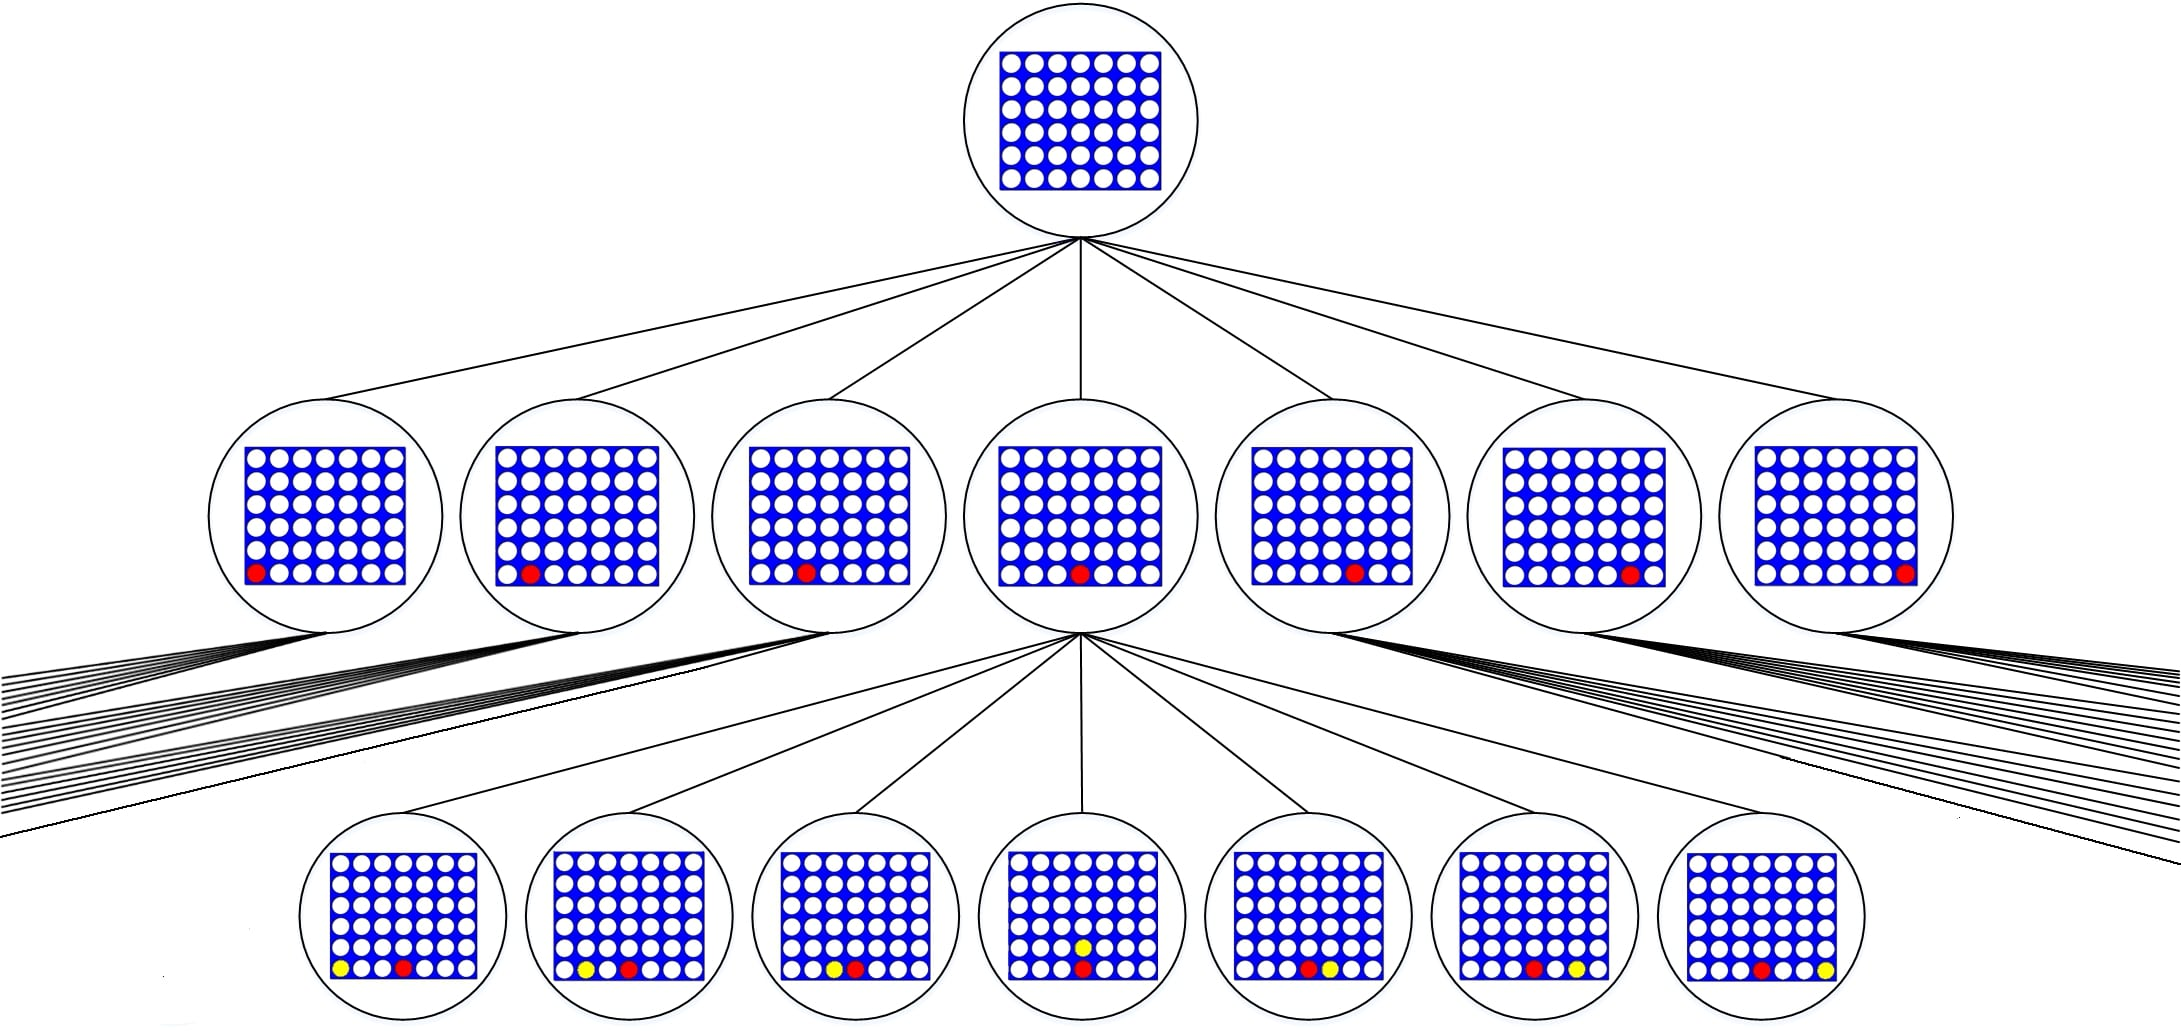
\includegraphics[scale=0.18]{tt.jpg}}

\caption{Espace de recherche du Puissance 4} 
\end{figure} 


L'illustration ci-dessus constitue l'espace de recherche du Puissance 4.
\\L'espace en question n'est pas complet sur l'illustration concernée puisque le nombre de possibilités est bien plus élevé suivant les coups joués par un joueur donné. Il y a en effet au départ sept configurations existantes pour le coup joué par le premier joueur (jeton rouge). 

On retrouve aussi sept configurations possibles pour le coup joué par le premier joueur dans les six autres états de jeu existants en partant du sommet de l'espace de recherche, ils ne sont pas représentés sur l'illustration précédente.

L'image ci-dessous représente les configurations possibles pour le premier état de jeu en partant du sommet. La démarche reste la même pour les autres états de jeu.

\begin{figure}[!h]
\centering
\fbox{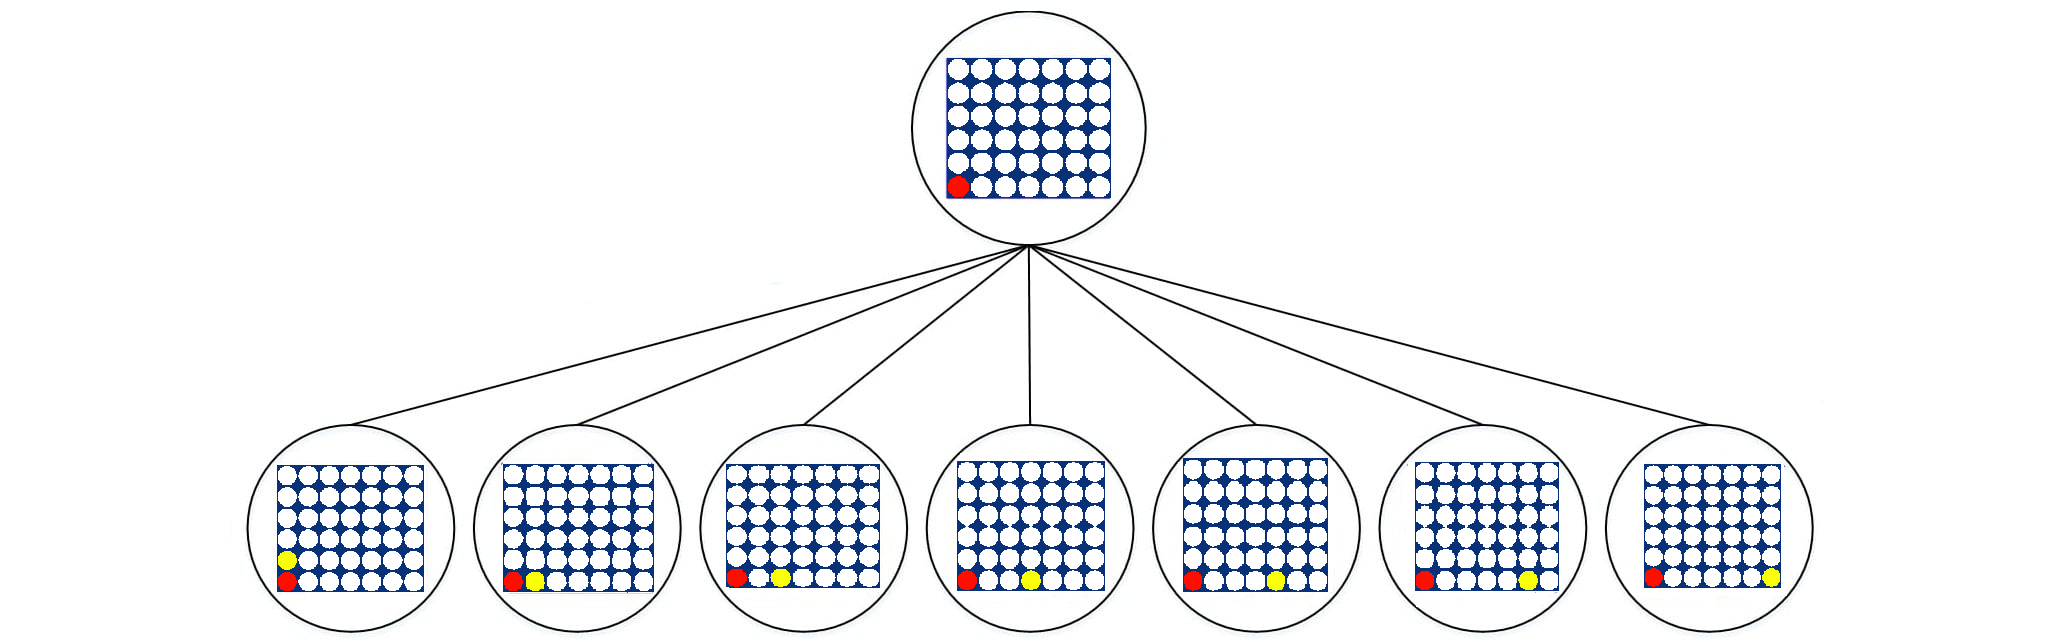
\includegraphics[scale=0.19]{fig3.png}}

\caption{Configurations possibles 1er état de jeu} 
\end{figure} 

\newpage

Il est alors question ici, d'envisager une autre approche algorithmique qui est celle de la méthode de \textbf{Monte-Carlo}.
La méthode de Monte-Carlo désigne au sens large une famille de méthodes algorithmiques, visant à calculer une valeur numérique approchée en faisant appel à des techniques dites "probabilistes".
Le nom de cette méthode fait allusion aux jeux de hasard pratiqués au Casino de Monte-Carlo situé à Monaco.




Cette méthode a été dévelopée dans les années 1950 par un groupe de chercheurs menés par \textit{Nicholas Metropolis}




\begin{figure}[!h] 
\centering
\fbox{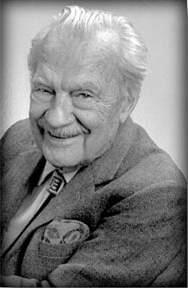
\includegraphics[width=1.8cm,scale=0.5]{Metropolis.png}}
\caption{Nicholas Metropolis} 
\end{figure} 


On retrouve la méthode de Monte-Carlo dans plusieurs domaines d'étude :

\vspace{0.4cm}

\begin{itemize}
\item Finance (estimation de la probabilité de la performance en bourse)
\item Mathématiques (détermination de la valeur du nombre $\pi$ / calcul d'intégrales) 
\item Algorithmique (estimation de la valeur d'un coup au jeu de Go / estimation de la valeur d'un coup aux échecs)

\end{itemize}






\subsection{Une approche simplifiée}

L'approche de Monte-Carlo est utilisée dans plusieurs jeux tour par tour tels que les échecs, le jeu de Go et le Puissance 4. L'approche classique du Monte-Carlo consiste simplement à limiter la profondeur de l'espace d'exploration qui sera représentée par un arbre de recherche, en étudiant les positions après un nombre de coups fixés.
Les feuilles de l'arbre de recherche correspondent précisément à une position terminale du jeu. 
Pour le Puissance 4, il y a 3 positions terminales possibles :
\vspace{0.2cm}

\begin{itemize}

	\item Victoire de l'IA
	\item Match Nul se traduisant par une saturation de la grille
	\item Victoire de l'humain

\end{itemize}

Cette approche consiste ainsi à explorer de façon systématique une branche de l'arbre de recherche jusqu'à une feuille (position terminale). Étant donné le nombre astronomique de parties possibles, cette approche ne peut pas explorer exhaustivement toutes les possibilités : il faut choisir un sous-ensemble des parties possibles

En partant du principe de l'exploration partielle d'un arbre de recherche jusqu'aux feuilles, l'implémentation d'un algorithme Monte-Carlo efficace doit répondre à deux problèmes :

\begin{itemize}

\item Le choix des séquences à explorer : Comment choisir celles qu'on explore ?
\item L'évaluation des coups joués : Comment déterminer le meilleur coup possible après une succession de coups joués ? 

\end{itemize}

\subsection{Stratégie et recherche arborescente MCTS Monte-Carlo Tree Search}

A partir d’une situation donnée, on joue une partie jusqu’à une situation finale (gain, perte ou une égalité).
\\On choisit aléatoirement un noeud d'une branche de l'arbre.
\begin{itemize}

\item Pas d’heuristique utilisée pour trier les noeuds et élaguer l’arbre
\item L’IA joue contre elle-même un grand nombre de fois et mémorise les chemins statistiquement intéressants

\end{itemize}



\begin{figure}[!h] 
\centering
\fbox{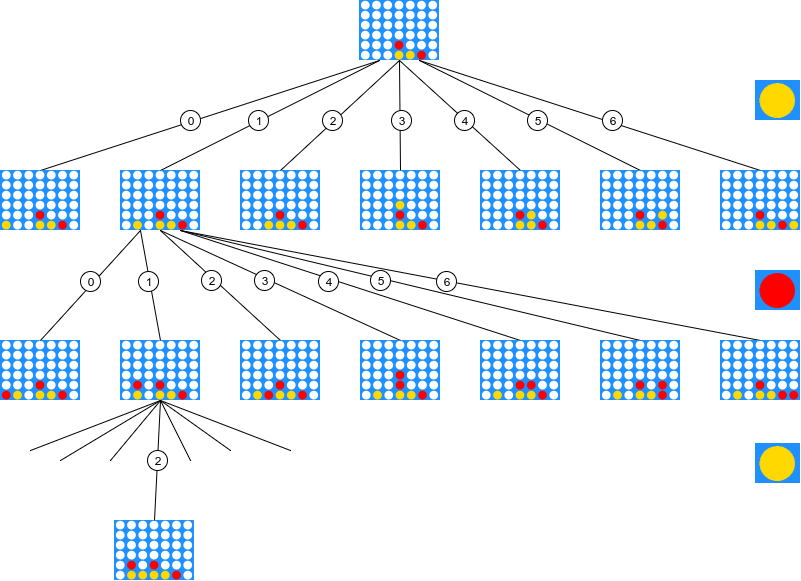
\includegraphics[scale=0.4]{MCTS.png}}
\caption{MCTS : Monte Carlo Tree Search} 
\end{figure}



L'illustration ci-dessus décrit l'arbre de jeu du Puissance 4. Il est question ici de comprendre les différentes phases sur lesquelles se base l'algorithme MCTS Monte-Carlo Tree Search.
On va notamment s’intéresser aux coups les plus prometteurs et aux coups sur lesquels on a le moins d’information. 
L’algorithme MCTS Monte-Carlo Tree Search peut se décomposer en 4 phases :
\vspace{0.4cm}

\begin{itemize}

\item (1) Sélection
\item (2) Expansion
\item (3) Simulation
\item (4) Rétropropagation 

\end{itemize}

\vspace{0.3cm}

La phase (1) va consister à déterminer quelles sous-branches de l’arbre sont intéressantes à explorer.
On peut partir par exemple de la racine de l'arbre et descendre progressivement pour voir quels coups sont les meilleurs parmi ceux qu’on aurait le plus envie de jouer (ceux qui ont le plus haut score).
Cette phase existe séparément de la phase suivante car souvent elle est associée à des heuristiques de jeu positionnelles.



\vspace{0.3cm}



Une fois les sous-branches sélectionnées, il sera question de choisir de façon aléatoire les n coups (étant pré-calculés pour maîtriser le temps de réponse) à développer linéairement.
Il s'agit ici de la phase d'\textbf{expansion}.

\vspace{0.3cm}

Durant la phase de \textbf{simulation}, on n’ajoute aucun nœud à l’arbre. On essaie juste de simuler une partie aléatoire aussi vite que possible pour obtenir un résultat rapidement. De plus, ajouter tous les nœuds à l’arbre le rendrait trop grand en mémoire et ajouterait des nœuds qu’on a choisi aléatoirement, alors que c’est précisément ce que l'on veut éviter.

\vspace{0.3cm}


Lorsque l'état final du jeu est atteint, on calcule le score des joueurs puis on le reporte sur les nœuds sélectionnés dans l’arbre, avec un pourcentage équivalent au nombre de fois où ils ont été sélectionnés. 
C’est ce que l'on appelle la \textbf{rétropropagation}.

L’algorithme MCTS Monte-Carlo Tree Search porte bien son nom car ce dernier revient à construire un arbre de recherche en utilisant l'algorithme de Monte Carlo.

Cet algorithme a vraiment été un important du point de vue de l’intelligence artificielle pour les jeux tour à tour. 
À une époque où les machines étaient incapables de jouer au jeu de go, l'algorithme MCTS Monte-Carlo Tree Search a permis de trouver un moyen autre que celui des fonctions d’évaluation et ainsi de progresser. 
Il a aussi donné un cadre dans lequel sont venus s’inscrire les algorithmes d’apprentissage.
On pourrait citer d'autres techniques d'apprentissage tels que le Q-learning ou le Deep Reinforcement Learning.

\vspace{0.2cm}

Les différentes phases de l'algorithme MCTS Monte-Carlo Tree Search peuvent être illustrées par le diagramme ci-dessous :

\begin{figure}[!h] 
\centering
\fbox{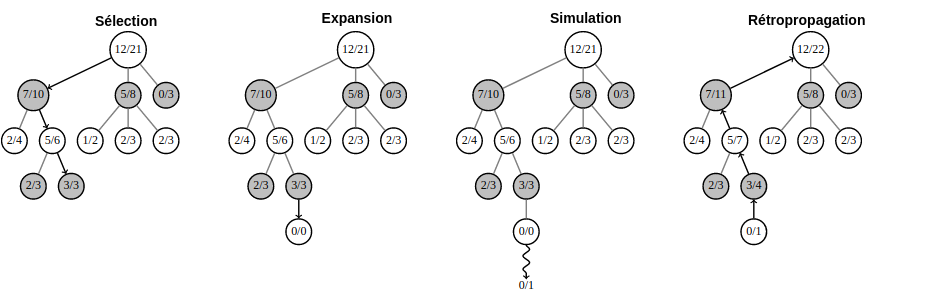
\includegraphics[scale=0.42]{mcts_sch.png}}
\caption{Diagramme MCTS} 
\end{figure}

\vspace{0.3cm}



\end{document}
